\documentclass[border=8pt]{standalone}
\usepackage{amsmath}
\usepackage{amssymb}
\usepackage{tikz}
\usetikzlibrary{arrows.meta,calc,decorations.pathreplacing,patterns,shapes.geometric,positioning,shadings,plotmarks}

\begin{document}
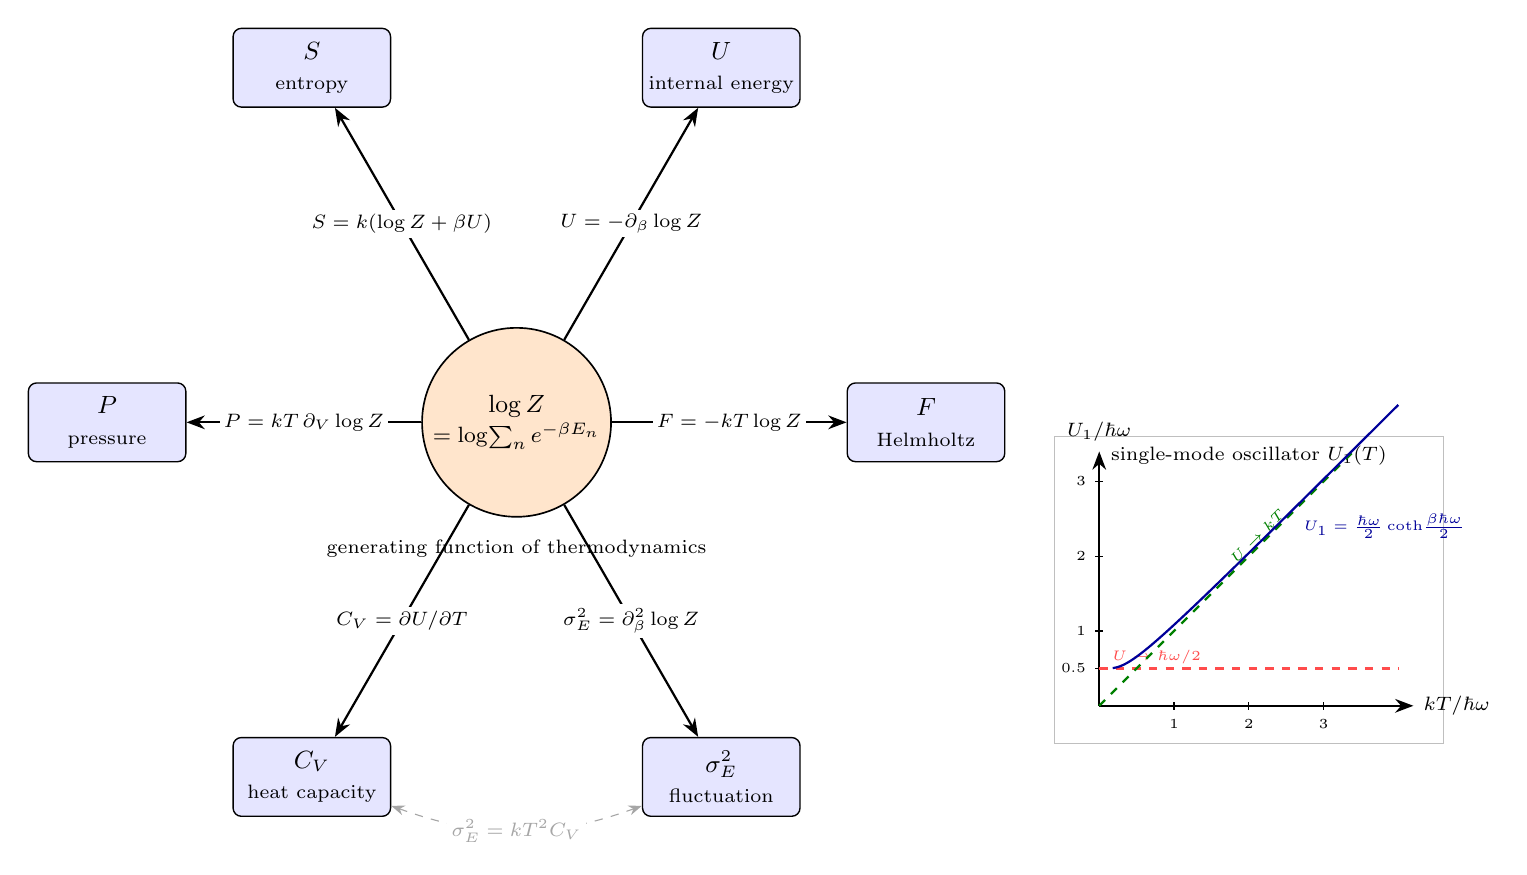
\begin{tikzpicture}[
  >=Stealth,
  font=\small,
  centernode/.style={circle, draw=black, fill=orange!20, minimum size=2.4cm, align=center, line width=0.6pt, inner sep=1pt},
  satnode/.style={rectangle, rounded corners=3pt, draw=black, fill=blue!10, minimum width=2.0cm, minimum height=1.0cm, align=center, line width=0.5pt, inner sep=2pt},
  arrowlbl/.style={font=\scriptsize, fill=white, inner sep=1.5pt},
  axis/.style={->, thick, black},
  curve/.style={blue!60!black, thick}
]

% --- Center node ---
\node[centernode] (Z) at (0,0) {$\log Z$ \\ {\footnotesize $=\log\!\sum_n e^{-\beta E_n}$}};

% --- Six surrounding nodes (hexagonal arrangement) ---
\node[satnode] (F) at (0:5.2)    {$F$ \\ \scriptsize Helmholtz};
\node[satnode] (U) at (60:5.2)   {$U$ \\ \scriptsize internal energy};
\node[satnode] (S) at (120:5.2)  {$S$ \\ \scriptsize entropy};
\node[satnode] (P) at (180:5.2)  {$P$ \\ \scriptsize pressure};
\node[satnode] (Cv) at (240:5.2) {$C_V$ \\ \scriptsize heat capacity};
\node[satnode] (Sg) at (300:5.2) {$\sigma_E^2$ \\ \scriptsize fluctuation};

% --- Arrows with labels ---
\draw[->, thick] (Z) -- (F)  node[arrowlbl, midway] {$F=-kT\log Z$};
\draw[->, thick] (Z) -- (U)  node[arrowlbl, midway] {$U=-\partial_\beta\log Z$};
\draw[->, thick] (Z) -- (S)  node[arrowlbl, midway] {$S=k(\log Z+\beta U)$};
\draw[->, thick] (Z) -- (P)  node[arrowlbl, midway] {$P=kT\,\partial_V\log Z$};
\draw[->, thick] (Z) -- (Cv) node[arrowlbl, midway] {$C_V=\partial U/\partial T$};
\draw[->, thick] (Z) -- (Sg) node[arrowlbl, midway] {$\sigma_E^2=\partial_\beta^2\log Z$};

% Connecting hint between Cv and sigma^2 (relation kT^2 C_V)
\draw[<->, dashed, gray!70] (Cv) to[bend right=20] node[arrowlbl, midway, fill=white] {$\sigma_E^2=kT^2 C_V$} (Sg);

% Center label below
\node[font=\scriptsize] at (0,-1.6) {generating function of thermodynamics};

% --- Inset: harmonic oscillator U(T) ---
\begin{scope}[shift={(7.4,-3.6)}, scale=0.95]
  % box
  \draw[gray!50, line width=0.3pt] (-0.6,-0.5) rectangle (4.6,3.6);
  \node[font=\scriptsize, anchor=north] at (2.0,3.6) {single-mode oscillator $U_1(T)$};
  % axes
  \draw[axis] (0,0) -- (4.2,0) node[right, font=\scriptsize] {$kT/\hbar\omega$};
  \draw[axis] (0,0) -- (0,3.4) node[above, font=\scriptsize] {$U_1/\hbar\omega$};
  % ticks x
  \foreach \x/\lab in {1/1, 2/2, 3/3} {
    \draw (\x,0.05) -- (\x,-0.05) node[below, font=\tiny] {\lab};
  }
  % ticks y
  \foreach \y/\lab in {0.5/0.5, 1/1, 2/2, 3/3} {
    \draw (0.05,\y) -- (-0.05,\y) node[left, font=\tiny] {\lab};
  }
  % low-T asymptote y=0.5
  \draw[red!70, dashed, thick] (0,0.5) -- (4.0,0.5);
  \node[red!70, font=\tiny, anchor=west] at (0.05,0.65) {$U\to\hbar\omega/2$};
  % high-T asymptote y=x
  \draw[green!50!black, dashed, thick] (0,0) -- (3.4,3.4);
  \node[green!50!black, font=\tiny, anchor=west, rotate=45] at (1.7,1.85) {$U\to kT$};
  % U(T) = (1/2) coth(1/(2x))  (in plotted units, U/hw vs kT/hw=x)
  \draw[curve, smooth, samples=80, domain=0.18:4.0]
    plot ({\x},{0.5*((exp(1/(2*\x))+exp(-1/(2*\x)))/(exp(1/(2*\x))-exp(-1/(2*\x))))});
  \node[curve, font=\tiny, anchor=west] at (2.6,2.4) {$U_1=\tfrac{\hbar\omega}{2}\coth\!\tfrac{\beta\hbar\omega}{2}$};
\end{scope}

\end{tikzpicture}
\end{document}
